\documentclass[a4paper,12pt]{article}
\usepackage[utf8]{inputenc}
\usepackage{graphicx}
\usepackage{amsmath}
\usepackage{amssymb}
\usepackage{pdfpages}
\usepackage[T1]{fontenc}
\usepackage{hyperref}
\usepackage{geometry}
\geometry{a4paper, margin=1in}

\usepackage{graphicx}
\usepackage{booktabs}
\usepackage{float}
\usepackage{listings}
\usepackage[x11names]{xcolor}

\lstdefinestyle{mystyle}{
    backgroundcolor=\color{white},   % 背景颜色
    commentstyle=\color{green},           % 注释颜色
    keywordstyle=\color{blue},            % 关键字颜色
    numberstyle=\tiny\color{gray},        % 行号样式
    stringstyle=\color{purple},              % 字符串颜色
    basicstyle=\ttfamily\footnotesize,    % 基本字体
    breaklines=true,                      % 自动换行
    frame=single,                         % 代码框架
    numbers=left,                         % 显示行号
    captionpos=b,                         % 标题位置
    showstringspaces=false,               % 不显示字符串中的空格
    tabsize=4,                              % 设置制表符宽度
    breaklines = true
}

\lstset{style=mystyle}  




\title{XL-Scanner}\date{}
\begin{document}
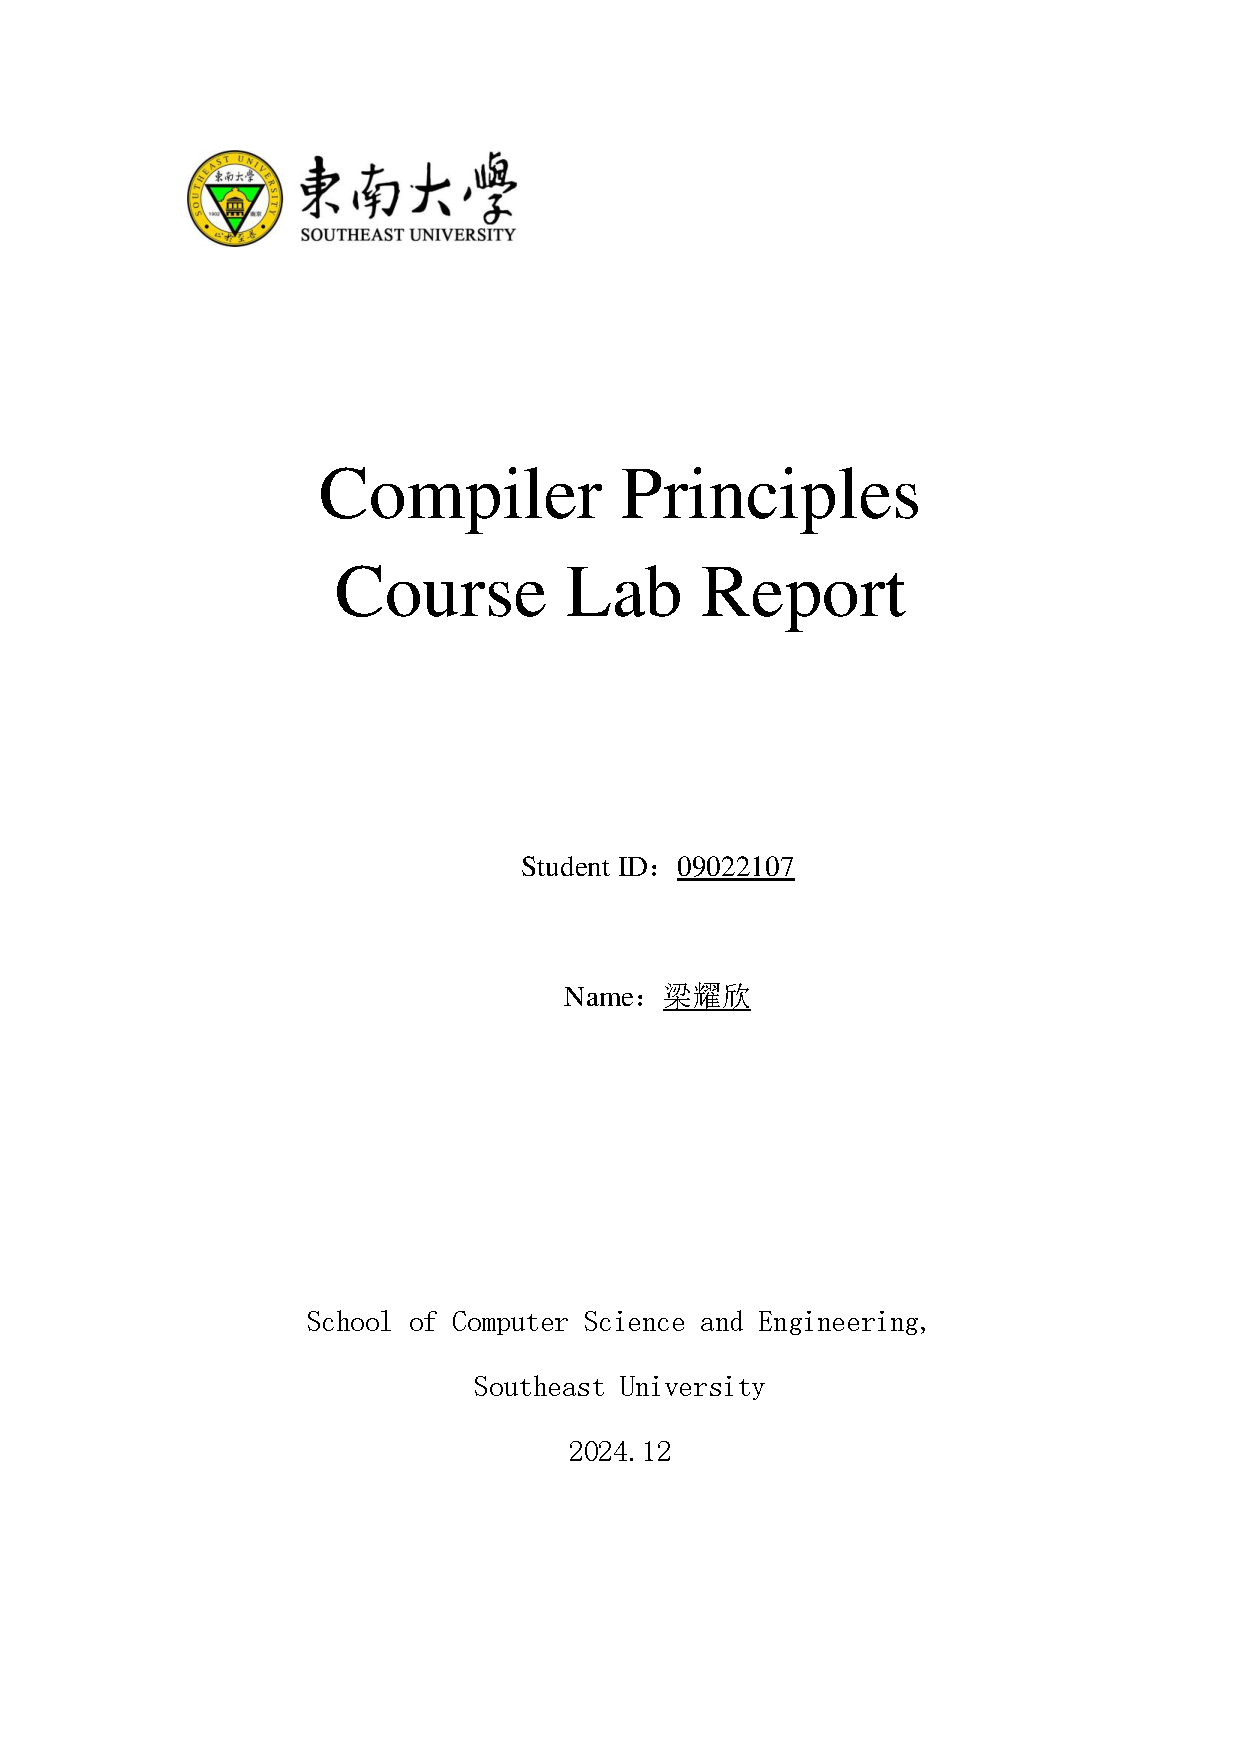
\includepdf[pages=1]{coverage.pdf} 
% 插入目录
\tableofcontents
\newpage
\maketitle



\section{Motivation/Aim}
The aim is to deepen the understanding of the lexical analysis process by writing a lexical analysis program.

\section{Content description}
\subsection{Non - programming implementation part (Constructing DFA of self - defined language)}
\begin{itemize}
    \item Define regular expressions.
    \item Convert the regular expressions into multiple NFAs.
    \item Merge these NFAs to form an overall NFA.
    \item Transform the NFA into the minimum DFA.
\end{itemize}
\subsection{Programming implementation part (Programming based on DFA)}
The lexical analysis program scans the test program character by character from left to right, generates triples of words (recognized string, word category, word category number), and outputs them to the result file. 

\section{Ideas/Methods}
\subsection{Idea}
The overall idea is to build a lexical analyzer to parse the content in the input text file (test.txt) according to lexical rules, split the text into different types of lexical units, and process and record relevant information for each type of lexical unit, thus providing processed basic data for subsequent compilation stages. By identifying different character combinations and symbol features, keywords, identifiers, numbers, strings, operators, etc. are distinguished, and comment content is properly handled to eliminate its interference with lexical analysis.
\subsection{Method}
\subsubsection{Classification and identification of lexical units}
Define the rules corresponding to various lexical units such as keywords and operators in advance. For example, keywords are listed through the predefined KEY\_WORDS array, and operators are listed through the OPERATORS array. When reading characters later, match and compare the character composition with these predefined contents to determine the type of lexical unit. In the judge\_str function, the type of lexical unit is preliminarily screened by judging the characteristics of the first character or the first few characters read. For example, those starting with letters may be keywords or identifiers, those starting with numbers are likely to be of the number type, those starting with " are likely to be strings, and those starting with // or /* correspond to different types of comments. According to these starting characteristics, different functions are called for further precise judgment and processing.
\subsubsection{Data storage and management}
Create data structures of type map<string, mpair> such as flag\_table (identifier table), num\_table (number table), and str\_table (string table) to store identifiers, numbers, strings, and their related information (the category number and number value in the table are saved in the form of mpair). Each time a lexical unit of the corresponding type is encountered, first check whether it already exists in the corresponding table. If it exists, obtain the existing number value. If it does not exist, add a new record and assign a new number value to manage the lexical unit information, facilitating subsequent query and repeated judgment operations.
\subsubsection{Comment processing}
The handle\_single\_comment function is used to directly ignore characters as comment content until a newline character or the end of the file is encountered after encountering content starting with //. In the handle\_multi\_comment function, once content starting with /* is identified, characters are read cyclically, and after encountering *, the next character is checked to see if it is / to determine whether the multi - line comment ends. All characters between /* and */ are ignored as comment parts to ensure that multi - line comments can be correctly processed without affecting the analysis of other lexical units.

The main function guides the entire lexical analysis process. First, try to open the input file. If it is successfully opened, read the file content character by character, filter out blank characters (spaces, tabs, newline characters), and call the judge\_str function for non - blank characters to further distinguish lexical units and perform corresponding processing until the file is read completely. Finally, close the file to complete the comprehensive lexical analysis task of the input text.

\section{Assumptions}
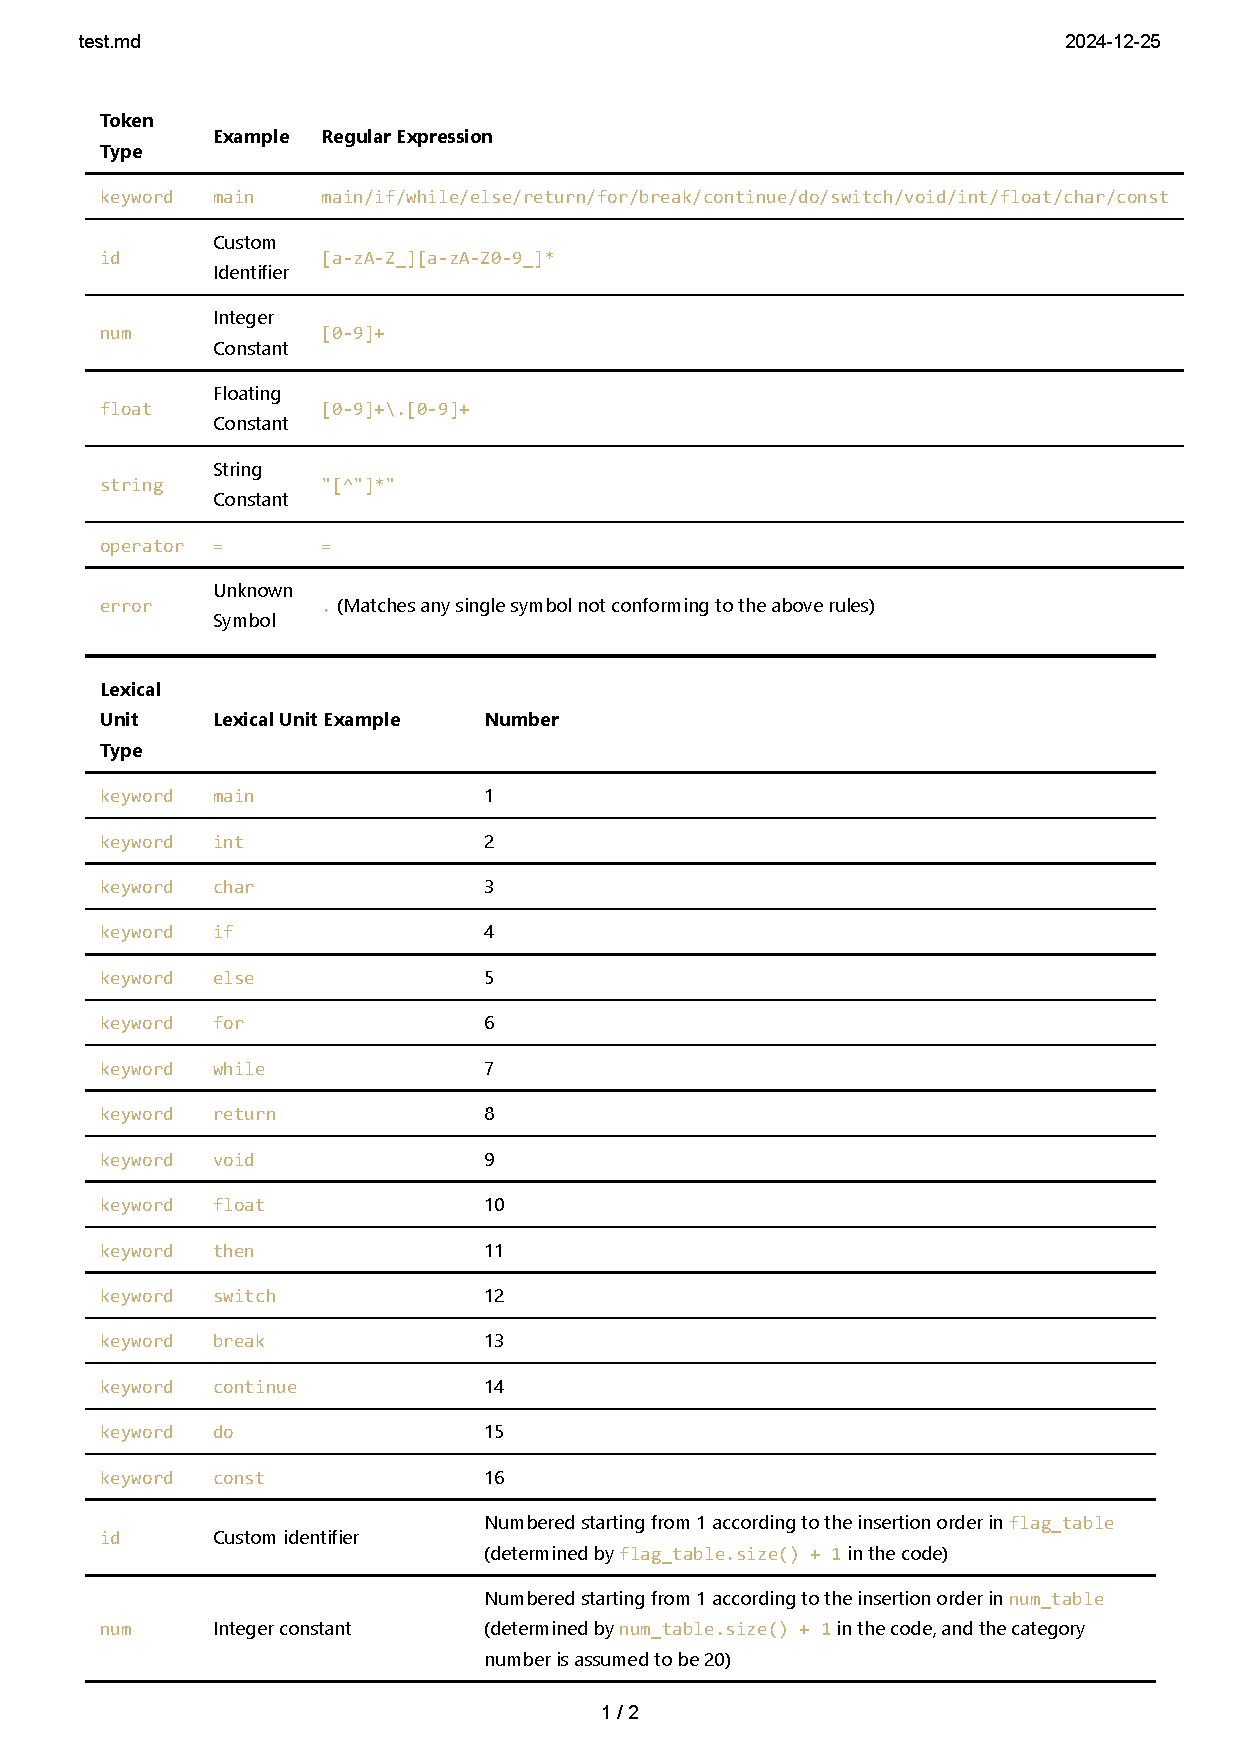
\includepdf[pages=1]{test.pdf}
\includepdf[pages=2]{test.pdf}

\section{Related FA descriptions}
The state transition diagram:

\vspace{10pt}
\centerline{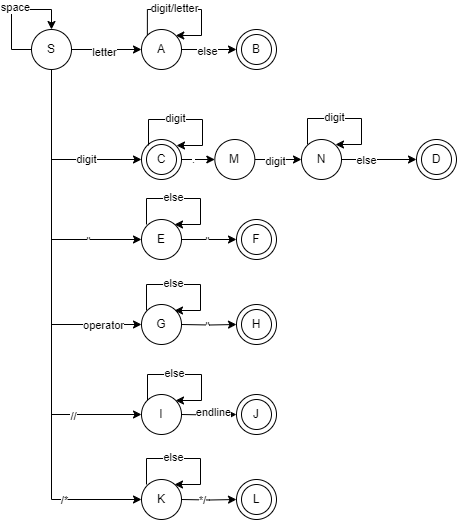
\includegraphics[width=0.6\textwidth]{photo/1.png}}
\vspace{10pt}

\section{Description of important Data Structures}
\begin{itemize}
    \item mpair (typedef pair<int, int> mpair;)
    It is a custom type alias used to combine two integer values. The first integer is used to represent the word category, and the second integer is used to represent the value of the word itself.
    \item map<string, mpair> (flag\_table, num\_table, str\_table)
    flag\_table (identifier table) is used to store the identifiers in the program. When an identifier is encountered, if the identifier is not in this table, the program will add it to the table and record the category information and position of the identifier in the table. If the identifier already exists in the table, relevant information can be quickly obtained through lookup operations.
    num\_table (number table) is used to store the numbers appearing in the program. When encountering a number, this table can distinguish different types of numbers such as integers and floating - point numbers, and record the position of each number in the table and its corresponding category information.
    str\_table (string table) is used to store the strings in the program. When encountering a string, the program will look up or add the string and its related category and position information in this table.
    \item Character arrays
    KEY\_WORDS stores a list of keywords in the program, including "main", "int", "char", "if", "else", "for", "while", "return", "void", "float", "then", "switch", "break", "continue", "do", "const". The input string is compared with the elements in this array one by one to determine whether the input string is a keyword.
    OPERATORS stores a list of operators, including "=", "+", "-", "*", "/", "(", ")", "[", "]", "{", "}", ",", ":", ";", ">", "<", ">=", "<=", "==", "\"". It is used to determine whether the input character is an operator.
\end{itemize}

\section{Description of core Algorithms}
\subsection{Lexical unit judgment functions}
\subsubsection{iskey function}
\begin{lstlisting}[language=c++]
int iskey(char* str)
{
    int len = sizeof(KEY_WORDS) / sizeof(char*);
    for (int i = 0; i < len; i++) {
        if (!strcmp(KEY_WORDS[i], str)) {
            return i;
        }
    }
    return -1;
}
\end{lstlisting}
Function: Determine whether the input string is a keyword.
Implementation: Traverse the KEY\_WORDS array and use the strcmp function to compare the input string with the elements in the keyword array one by one. If a match is found, return the index of the keyword in the array, otherwise return - 1.

\subsubsection{isope function}
\begin{lstlisting}[language=c++]
int isope(char* str)
{
    int len = sizeof(OPERATORS) / sizeof(char*);
    for (int i = 0; i < len; i++) {
        if (!strcmp(OPERATORS[i], str)) {
            return i;
        }
    }
    return -1;
}
\end{lstlisting}
Function: Determine whether the input string is an operator.
Implementation: Traverse the OPERATORS array and use the strcmp function to compare the input string with the elements in the operator array one by one. If a match is found, return the index of the operator in the array, otherwise return - 1.

\subsubsection{isFloatPart function}
\begin{lstlisting}[language=c++]
bool isFloatPart(char ch)
{
    int asciiCode = static_cast<int>(ch);
    return (asciiCode == 46 || asciiCode == 101 || asciiCode == 69 || isdigit(static_cast<int>(ch)));
}
\end{lstlisting}
Function: Assist in determining whether a character may be part of a floating - point number.
Implementation: Determine whether the character is., e, E, or a digit by judging the ASCII code value of the character.

\subsection{Lexical unit acquisition functions}
\subsubsection{get\_keyorid function}
\begin{lstlisting}[language=c++]
void get_keyorid(char* token, char* ptr, FILE* fp)
{
    while (isalnum(*ptr)) {
        *++ptr = fgetc(fp);// Read letters or numbers
    }
    ungetc(*ptr, fp);// If no letters or numbers are read, return a string ending with \0, that is, a token
    *ptr = '\0';
    int flag = iskey(token);
    if (flag!= -1) { // It is a keyword
        if (!mark_key[flag])
            mark_key[flag] = 1;
        cout << "(" << token << ",keyword," << flag + 1 << ")" << endl;
    }
    else { // It is an identifier
        string s = "";
        map<string, mpair>::iterator it;
        s.append(token);
        it = flag_table.find(s);
        mpair mp;
        if (it == flag_table.end()) { // The identifier is not in the symbol table
            mp = make_pair(10, flag_table.size() + 1);// Create an mpair object
            flag_table[s] = mp;
            cout << "(" << s << ",id," << flag_table.size() << ")" << endl;
        }
        else {
            it = flag_table.find(s);
            mp = it->second;
            cout << "(" << s << ",id," << mp.second << ")" << endl;
        }
    }
}
\end{lstlisting}
Function: Get keywords or identifiers.
Implementation: When the input character is a letter, continuously read subsequent characters until they are not letters or numbers, and form a string token from the read characters. Then call the iskey function to determine whether it is a keyword. If it is a keyword, record relevant information and output it. If it is not a keyword, treat it as an identifier. According to the identifier table flag\_table, determine whether the identifier already exists. If it does not exist, add it to the table, record relevant information, and output it. If it exists, directly output the existing relevant information in the table.

\subsubsection{get\_number function}
\begin{lstlisting}[language=c++]
void get_number(char* token, char* ptr, FILE* fp)
{
    bool isFloat = false;  // Mark whether it is a floating - point number
    while (isdigit(*ptr) || (isFloatPart(*ptr) &&!isFloat)) {
        if (*ptr == '.' || *ptr == 'e' || *ptr == 'E') {
            isFloat = true;
        }
        *++ptr = fgetc(fp);
    }
    ungetc(*ptr, fp);
    *ptr = '\0';

    map<string, mpair>::iterator it;
    string num;
    num.append(token);
    it = num_table.find(num);
    mpair mp;
    if (it == num_table.end()) {
        if (isFloat) {
            mp = make_pair(30, num_table.size() + 1);  // Assume the category number of floating - point numbers is 30, which can be adjusted according to the actual situation
        }
        else {
            mp = make_pair(20, num_table.size() + 1);
        }
        num_table[num] = mp;
    }
    else {
        it = num_table.find(num);
        mp = it->second;
    }
    string sub;
    if (num.length() > width1 - 1) {
        sub = num.substr(0, width1 - 4);
        sub.append("...");
    }
    else
        sub = num;
    if (isFloat) {
        cout << "(" << num << ",float," << mp.second << ")" << endl;
    }
    else {
        cout << "(" << num << ",num," << mp.second << ")" << endl;
    }
}
\end{lstlisting}
Function: Get numbers (including integers and floating - point numbers).
Implementation: When the input character is a number, continuously read subsequent characters, determine whether it is a floating - point number according to the isFloatPart function, until the read character does not conform to the rules of numbers or floating - point numbers. Form a string num from the read characters, then determine whether the number already exists according to num\_table. If it does not exist, add it to the number table according to whether it is a floating - point number, record relevant information, and output it. If it exists, directly output the existing relevant information in the table.

\subsubsection{try\_string function}
\begin{lstlisting}[language=c++]

void try_string(char* token, char* ptr, FILE* fp)
{
    *++ptr = fgetc(fp);
    while (!feof(fp) && *ptr!= '"') {
        *++ptr = fgetc(fp);
    }
    if (!feof(fp)) // Haven't reached the end of the file
        *++ptr = '\0';
    else // Have reached the end of the file
        *ptr = '\0';
    string s = "", sub;
    s.append(token);
    if (s.size() > 0) {
        if (*(ptr - 1) == '"') { // Found the matching "
            map<string, mpair>::iterator it;
            it = str_table.find(s);
            mpair mp;
            if (it == str_table.end()) {
                mp = make_pair(50, str_table.size() + 1);
                str_table[s] = mp;
                cout << "(" << s << ",string," << str_table.size() << ")" << endl;
            }
            else {
                it = str_table.find(s);
                mp = it->second;
                cout << "(" << s << ",string," << mp.second << ")" << endl;
            }
        }
        else { // Didn't find the matching "
            int i;
            int len = strlen(token);
            for (i = 0; i < len - 1; i++)
                ungetc(*--ptr, fp);
            cout << "(" << s << ",error,miss terminal '\"')" << endl;
        }
    }
}
        \end{lstlisting}
        Function: Determine whether it is a string.
        Implementation: When the input character is a double quotation mark ("), continuously read subsequent characters until the next double quotation mark is encountered or the end of the file is reached. If a matching double quotation mark is encountered, then determine whether the string already exists in the \texttt{str\_table}. If it does not exist, add it to the table and record relevant information and then output it. If it exists, directly output the existing relevant information in the table. If a matching double quotation mark is not encountered, then perform error handling and output an error message.
        
        \subsubsection{try\_double\_ope Function}
        \begin{lstlisting}[language=c++]
void try_double_ope(char* token, char* ptr, FILE* fp)
{
    *++ptr = fgetc(fp);
    *++ptr = '\0';
    int sub = isope(token);
    if (sub!= -1)
        mark_ope[sub] = 1;
    else {
        ungetc(*--ptr, fp);
        *ptr = '\0';
        sub = isope(token);
        mark_ope[sub] = 1;
    }
    cout << "(" << token << ",operator," << sub + 21 << ")" << endl;
}
        \end{lstlisting}
        Function: Process possible double - operand operators.
        Implementation: When the input character is one of the possible starting characters of double - operand operators such as >, <, or =, read the next character to form a string \texttt{token}, and call the \texttt{isope} function to determine whether it is an operator. If it is, record relevant information and output it. If it is not, return the second character to the input stream and re - judge the first character as a single - operand operator.
        
        \subsubsection{try\_single\_ope Function}
        \begin{lstlisting}[language=c++]
void try_single_ope(char* token, char* ptr, FILE* fp)
{
    *++ptr = '\0';
    int sub = isope(token);
    if (sub!= -1) {
        mark_ope[sub] = 1;
        cout << "(" << token << ",operator," << sub + 21 << ")" << endl;
    }
    else {
        if (token[0] < 0 || token[0] > 127) // Non - ASCII code
            token[0] = '?';
        cout << "(" << token << ",error,unknown symbol)" << endl;
    }
}
        \end{lstlisting}
        Function: Process single - operand operators.
        Implementation: When the input character is an operator and not the starting character of a double - operand operator, call the \texttt{isope} function to determine whether it is an operator. If it is, record relevant information and output it. If it is not and the character is a non - ASCII code, then perform error handling and output an error message.
        
\subsection{Comment Processing Functions}
        \subsubsection{handle\_single\_comment Function}
        \begin{lstlisting}[language=c++]
void handle_single_comment(FILE* fp)
{
    char ch;
    while ((ch = fgetc(fp))!= '\n' && ch!= EOF) {
        // Continuously read characters until a newline character or the end of the file is encountered
    }
}
        \end{lstlisting}
        Function: Process single - line comments.
        Implementation: When the input character is //, continuously read subsequent characters until a newline character or the end of the file is encountered.
        
        \subsubsection{handle\_multi\_comment Function}
        \begin{lstlisting}[language=c++]
void handle_multi_comment(FILE* fp)
{
    char ch;
    int comment_end_found = 0;
    while ((ch = fgetc(fp))!= EOF &&!comment_end_found) {
        if (ch == '*') {
            char next_ch = fgetc(fp);
            if (next_ch == '/') {
                comment_end_found = 1;
            }
            else {
                ungetc(next_ch, fp);
            }
        }
    }
}
        \end{lstlisting}
        Function: Process multi - line comments.
        Implementation: When the input character is /*, continuously read subsequent characters until */ is encountered or the end of the file is reached.
        
\subsection{Lexical Analysis Loop in the main Function}
        \begin{lstlisting}[language=c++]
void judge_str(char ch, FILE* fp)
{
    char token[TOKEN_SIZE];
    char* ptr = token;
    *ptr = ch;
    char next_char = fgetc(fp);// Read the next character for auxiliary judgment
    ungetc(next_char, fp);// Immediately return to prevent affecting the reading

    if (isalpha(*ptr)) { // The token starts with a letter
        get_keyorid(token, ptr, fp); // Determine whether it is a keyword or an identifier
    }
    else if (isdigit(*ptr)) { // The token starts with a number
        get_number(token, ptr, fp); // Determine whether it is a number
    }
    else if (*ptr == '"') { // The token starts with "
        try_string(token, ptr, fp); // It may be a string
    }
    else if (*ptr == '>' || *ptr == '<' || *ptr == '=') { // It may be a double - operand operator
        try_double_ope(token, ptr, fp);
    }
    else if (*ptr == '/' && next_char == '/') { // Starts with "//", process single - line comments
        handle_single_comment(fp);
    }
    else if (strncmp(COMMENT_START_MULTI, ptr, 2) == 0) { // Starts with "/*", process multi - line comments
        handle_multi_comment(fp);
    }
    else {
        try_single_ope(token, ptr, fp); // It may be a single - operand operator
    }
}
int main()
{
    FILE* fp = fopen("test.txt", "r");
    if (fp == NULL) {
        perror("file open failed\n");
        return 1;
    }
    char ch = fgetc(fp);
    while (!feof(fp)) {
        if (ch!= ' ' && ch!= '\t' && ch!= '\n') {
            judge_str(ch, fp);
        }
        ch = fgetc(fp);
    }
    fclose(fp);
    cout << "---------------------------------------" << endl;
    // Output the identifier table
    cout << "identifier table:" << endl;
    for (auto& it : flag_table) {
        cout << it.second.second << "   " << it.first << endl;
    }

    // Output the integer table
    cout << "num table:" << endl;
    for (auto& it : num_table) {
        if (it.second.first == 20) {
            cout << it.second.second << "   " << it.first << endl;
        }
    }

    // Output the floating - point table
    cout << "float table:" << endl;
    for (auto& it : num_table) {
        if (it.second.first == 30) {
            cout << it.second.second << "   " << it.first << endl;
        }
    }

    return 0;
}
        \end{lstlisting}
        In the \texttt{main} function, the file \texttt{test.txt} is opened and its content is read character by character. When the read character is not a space, tab, or newline character, the \texttt{judge\_str} function is called for lexical analysis. The \texttt{judge\_str} function calls the corresponding lexical unit acquisition functions or comment processing functions according to the type of the input character. When the file reading is completed (judged by the \texttt{feof} function), the file is closed and the program ends.
        
\section{Use Cases on Running}
        The following \texttt{test.cpp} file is used for code testing, and the results are output in the form of triples:
        \begin{lstlisting}[language=c++]
int num1 = 123;
float num2 = 3.14;
char str1 = "Hello, World!";
if (num1 > 100) {
    int num3 = 456;
    return num3;
} else {
    continue;
}
&
// This is a single-line comment
/* This is a
multi-line
comment */
        \end{lstlisting}
        The output is:
        
        \begin{lstlisting}
identifier table:
5   This
7   a
10   comment
6   is
9   line
8   multi
1   num1
2   num2
4   num3
3   str1
num table:
3   100
1   123
4   456
float table:
2   3.14
        \end{lstlisting}
The output file test.txt:

\vspace{10pt}
\centerline{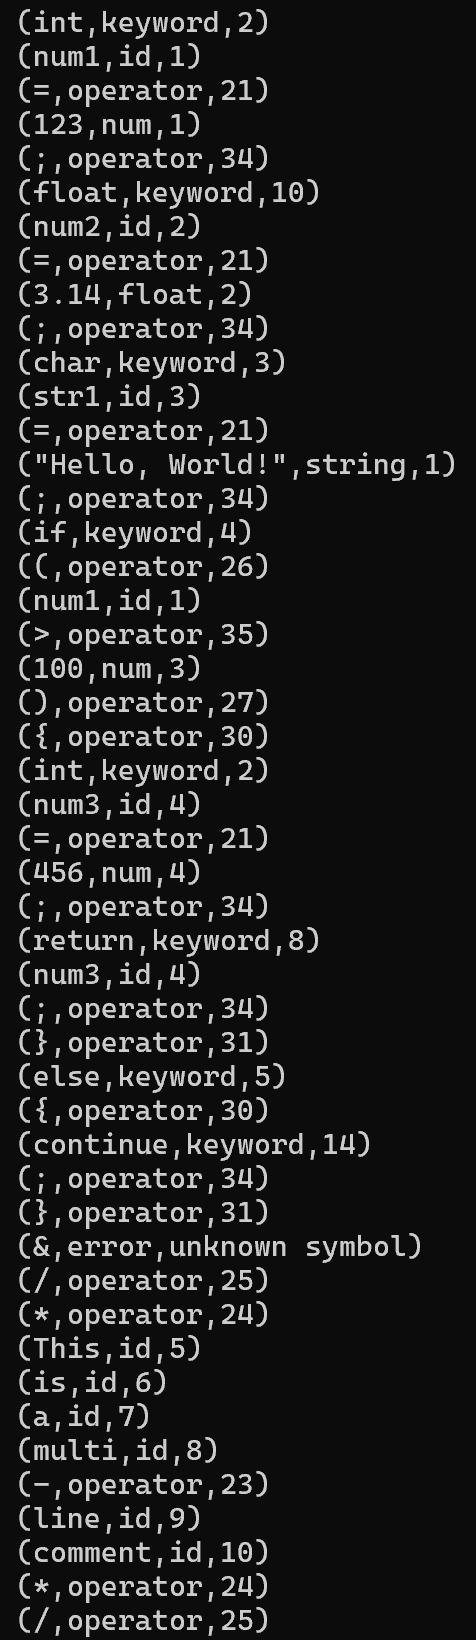
\includegraphics[width=0.3\textwidth]{photo/2.png}}
\vspace{10pt}


\section{Problems Occurred and Related Solutions}
At first, the judgment of / was not very clear. Later, a method was found. When // was recognized as the start of a single - line comment, a special state flag was set to enter the single - line comment processing state. In this state, no matter what characters were encountered subsequently (except for the newline character as the end mark), they were directly ignored until the newline character was encountered and then exited this state to return to the normal lexical analysis state. For the multi - line comment /* */, a corresponding state was also set. After entering the multi - line comment state, characters were continuously read, and only when */ was read in sequence would the state be exited to return to the normal analysis state. And some error handling mechanisms could be added. For example, if the end of the file was reached without encountering */, an appropriate error message could be output to inform the user that the comment was not correctly closed. In addition, for the case where the string originally contained escape characters, the initial program might prematurely consider the double quotation mark as the end, resulting in the truncation of the string. The loop logic in the \texttt{try\_string} function was modified. When the backslash \ character was read, it was necessary to additionally determine whether the next character was a specific character used for escape (such as the case where \ was followed by "). If it was an escape character combination, it was normally read as part of the string content instead of being treated as the end double quotation mark, so that the string content containing escape characters could be correctly parsed.

\section{Feelings and Comments}
(1) By writing a lexical analyzer, I have a deeper understanding of the compilation process. Lexical analysis is the first stage of compilation, which needs to convert the source code text into a series of tokens, maintain a symbol table to record the encountered self - defined identifiers and some constants, and also needs to complete the error detection function to identify lexical errors in the source code, such as spelling errors and illegal characters.

(2) Before writing a lexical analyzer, it is necessary to draw a state transition diagram first and write processing functions for different situations according to the state transition diagram. The basis for drawing the state transition diagram is to divide the read characters into different categories and determine which category they belong to according to the first character, and then specifically analyze the possible read characters for different categories.
    \end{document}        